%! suppress = TooLargeSection
\documentclass[a4paper,11pt]{article}%Schriftgröße
\usepackage[T1]{fontenc}
\usepackage[utf8]{inputenc}
\usepackage[ngerman]{babel}%Veröffentlichungssprache
\usepackage{graphicx}
\usepackage{ragged2e}
\usepackage[format=plain,justification=RaggedRight,singlelinecheck=false,font={small},labelsep=space]{caption}
\usepackage{xcolor}
\definecolor{th_red}{rgb}{0.9,0.1,0.1}

\usepackage[a4paper]{geometry}
\geometry{left=3.5cm,right=2.5cm,top=2.4cm,bottom=2cm}%Seitenränder
\usepackage[onehalfspacing]{setspace}%Zeilenabstand
\renewcommand{\\}{\vspace*{0.5\baselineskip} \newline}
\renewcommand*\MakeUppercase[1]{#1}
\usepackage{fancyhdr}
\pagestyle{fancy}
\renewcommand{\headrulewidth}{0pt}
\renewcommand{\footrulewidth}{0pt}
\fancyhead[R]{\footnotesize{\thepage}}
%\fancyhead[L]{\footnotesize{\leftmark}}
\fancyfoot{}
\usepackage[colorlinks,
    pdfpagelabels,
    pdfstartview = FitH,
    bookmarksopen = true,
    bookmarksnumbered = true,
    linkcolor = th_red,
    urlcolor = th_red,
    plainpages = false,
    hypertexnames = false,
    citecolor = black] {hyperref}
\usepackage{pdfpages}

\begin{document}
    \begin{titlepage}
        \begin{flushleft}
            \vspace*{-1cm}
            
\includegraphics[scale=1]{TH}\\
            \vspace*{1cm}
        \end{flushleft}
        \begin{huge}
            \noindent
            Praktische Evaluation des Frameworks
            \newline
            Laravel Nova am Beispiel einer Anwendung zur
            \newline
            Verwaltung und Auswertung von
            \newline
            Radiosondenaufstiegen
        \end{huge}
        \\
        Exposé im Rahmen des Praxisprojektseminars
        \newline
        an der Fakultät für Informatik und Ingenieurwissenschaften
        \newline
        der Technischen Hochschule Köln
        \\ \\ \\
        \noindent
        \begin{tabular}{ll}
            vorgelegt von:   & Niklas Canisius       \\
            Matrikelnummer:  & 11110023              \\
            Adresse:         & Gelpestraße 96        \\
            ~                & 51647 Gummersbach     \\
            ~                & niklas@canisius.email \\
            ~                & ~                     \\
            eingereicht bei: & Prof.\ Dr. Kohls      \\
            \\ \\ \\ \\ \\  \\ \\ \\ \\ \\ \\ \\ \\ \\ \\ \\ \\
            Gummersbach, \today
        \end{tabular}
    \end{titlepage}

    \pagenumbering{Roman}
    \pagestyle{fancy}

    \newpage


    \section{Problemfeld \& Kontext}
    Bisherige individuelle Projekte des Softwareunternehmens \href{https://kiwis-and-brownies.de}{Kiwis \& Brownies GbR} zeigten einen anfänglich großen und repetitiven Aufwand bei der Erstellung unterschiedlichster Software auf.
    Fast alle Projekte benötigen einen Login, die Verwaltung von Entitäten in einem sogenannten \href{https://www.educative.io/blog/crud-operations}{CRUD} Interface, verschiedene Auswertungen, sowie spezielle Abläufe für ein oder mehrere Entitäten.


    \section{Ziel}
    Im vorliegenden Projekt soll das Framework \href{https://nova.laravel.com}{Laravel Nova} verwendet werden, um den Aufwand der Entwicklung zu reduzieren, gleichzeitig aber keine Flexibilität bei der Umsetzung zu verlieren.
    Die Wahl des Frameworks ergab sich auf Basis von Erfahrungen im Unternehmen, sowie Kundenwünschen.
    Das System soll webbasiert und auf Basis von weit verbreiteten und möglichst quelloffenen Frameworks umgesetzt werden.
    Das Unternehmen hat in der Vergangenheit primär Kompetenzen in der Entwicklung mit \href{https://www.php.net}{PHP} und dem Framework \href{https://laravel.com}{Laravel} gesammelt, beide erfüllen die Projektanforderungen.
    Als First-Party Paket ist daher die Wahl auf Laravel Nova gefallen.


    \section{Aufgabenstellung}
    Die Hauptaufgabe liegt in der Implementation des Systems mit allen vorgegebenen Funktionalitäten (siehe Lastenheft und Leistungspaket im Anhang).
    Dabei soll sich zeigen, inwiefern Laravel Nova die Arbeit erleichtert und welche Einschränkungen sich ergeben.
    Außerdem könnte eine Literaturrecherche zeigen, ob es bisherige Arbeiten gibt, die eine ähnliche Problematik beleuchten.

    \subsection{Forschungsfrage}
    Welche Vor- und Nachteile bietet der Einsatz eines Administration-Panels am konkreten Beispiel von Laravel Nova?
    Verglichen wird mit einer Entwicklung auf Basis von Laravel, ohne Nova.


    \section{Lösungsansätze}
    Die Beantwortung der Forschungsfrage soll sich durch den praktischen Einsatz der Technologie an einem Projektbeispiel zeigen.
    Um das dabei gewonnene Fazit zu überprüfen, könnte in einer späteren Erweiterung, z.B.\ im Rahmen der Bachelorarbeit, ein weiteres Projekt oder Erweiterungen mit dem Framework umgesetzt werden.

    \newpage


    \section{Chancen \& Risiken}
    Der Einsatz des zu überprüfenden Frameworks bietet die Chance einer schnelleren und stringenteren Entwicklung der Software mit dem Fokus auf die wirkliche Anwendungslogik und nicht auf grundlegende Funktionalitäten/Bausteine beziehungsweise das Programmiergerüst.
    Ein mögliches Risiko hingegen ist die Einschränkung in der Umsetzung durch die fehlende Anpassbarkeit der Software.
    \\
    Problematisch ist der Projektkontext in einem Unternehmen.
    Hier kommt ein wichtiger Stakeholder mit ins Boot und daher gibt es möglicherweise im Laufe des Projektes Konflikte zwischen wirtschaftlichen und wissenschaftlichen Anforderungen.
    \\
    Ein Problem liegt außerdem in der Erarbeitung des Fazits.
    Es ist zu klären, nach welchen Metriken die Vor- und Nachteile erhoben werden und mit welcher Gewichtung sie in das Gesamtfazit eingehen.


    \section{Ressourcen, Setup \& Abhängigkeiten}
    Eine erste Literaturrecherche bei Google Scholar brachte nur wenige und nicht zufriedenstellende Ergebnisse.
    \newline
    \href{https://gitlab.com/graw-radiosondes/sounding-console/-/wikis/04-Research}{https://gitlab.com/graw-radiosondes/sounding-console/-/wikis/04-Research}
    \\
    Die Technologie ist bereits recht konkret festgelegt, Änderungen daran sind unwahrscheinlich und ergeben sich nur evtl. im laufenden Projekt.
    \\
    Prüfer und Betreuer an der Technischen Hochschule ist \textit{noch zu klären}.
    \\
    Kooperationspartner des Projektes ist die Kiwis \& Brownies GbR mit Sitz in Gummersbach.
    Verantwortlicher im Unternehmen ist Benjamin Braun und technischer Betreuer ist Keanu Buschbacher.
    \\
    Der Hauptteil der Arbeit wird bei Kiwis \& Brownies im Office oder Homeoffice absolviert.


    \section{Motivation}
    Persönlich motiviert mich die Herausforderung ein neues Framework kennenzulernen und einzusetzen.
    Zudem ergibt sich aus meiner bisherigen Arbeit im Unternehmen ein starkes Interesse an einem solchen Framework, da es unternehmensintern eine Eigenentwicklung gibt, die im Prinzip das gleiche Problemfeld bearbeitet.
    Daher könnte eine mögliche Folgearbeit, z.B.\ im Rahmen der Bachelorarbeit, der Vergleich der Beiden Lösungen \href{https://brezel.io}{Brezel} und \href{https://nova.laravel.com}{Laravel Nova} sein.
    \\
    Durch das Studium der Medieninformatik besitze ich die technischen Kompetenzen für die Entwicklung eines solchen Systems und bin interessiert diese einzusetzen.
    Vor allem die notwendigen Kompetenzen im Bereich Softwaretechnik und Webtechnologien, welche durch die entsprechenden Module im Schwerpunkt Web-Development vermittelt wurden.


    \section{Arbeitsergebnis}
    Das Ergebnis ist zum Hauptteil die Implementierung der Software sowie deren Dokumentation.
    Außerdem ist das Fazit über die Vor- und Nachteile des Frameworks ein zentrales Ergebnis der Arbeit.


    \section{Meilensteine}
    Die Meilensteine und ihre konkreten Aufgaben sind im privaten Repository bei GitLab definiert.
    Bei Bedarf wird Einsicht gewährt.
    \newline
    \href{hthttps://gitlab.com/graw-radiosondes/sounding-console/-/milestones}{https://gitlab.com/graw-radiosondes/sounding-console/-/milestones}
    \newline
    \href{hthttps://gitlab.com/graw-radiosondes/sounding-console/-/boards}{https://gitlab.com/graw-radiosondes/sounding-console/-/boards}


    \section{Sperrvermerk}
    Das vorliegende Dokument beinhaltet vertrauliche Daten der Firma Graw Radiosondes GmbH \& Co. KG sowie der Kiwis \& Brownies GbR\@.
    Es darf nur von berechtigten Personen innerhalb Ihrer dienstlichen Verpflichtungen eingesehen werden.
    Eine Veröffentlichung und Vervielfältigung – auch in Teilen – ist untersagt.
    Dritten darf dieses Dokument nur mit der ausdrücklichen Genehmigung des Verfassers und beider Unternehmen zugänglich gemacht werden.

    \newpage


    \section{Anhang}

    \subsection{Lastenheft}
    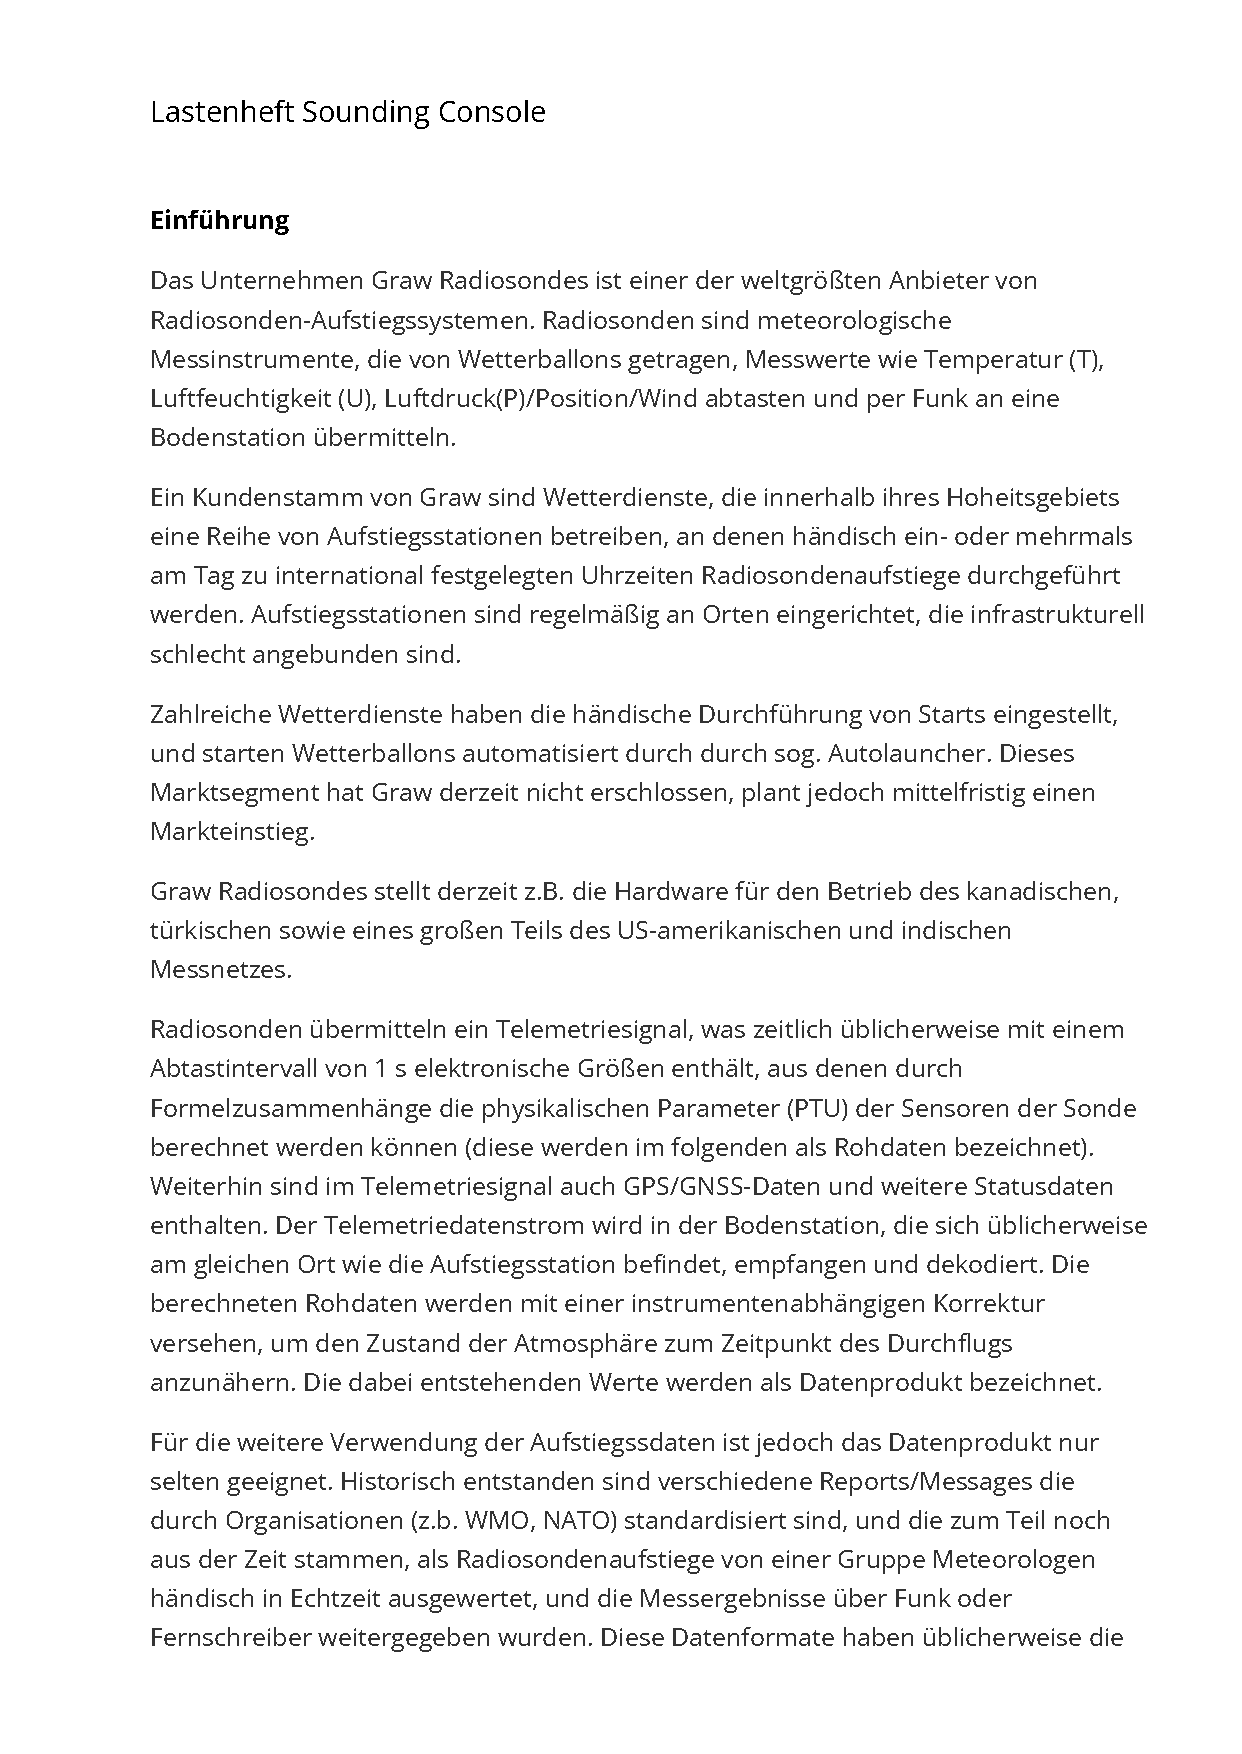
\includepdf[pages=-]{Lastenheft.pdf}

    \subsection{Leistungspaket}
    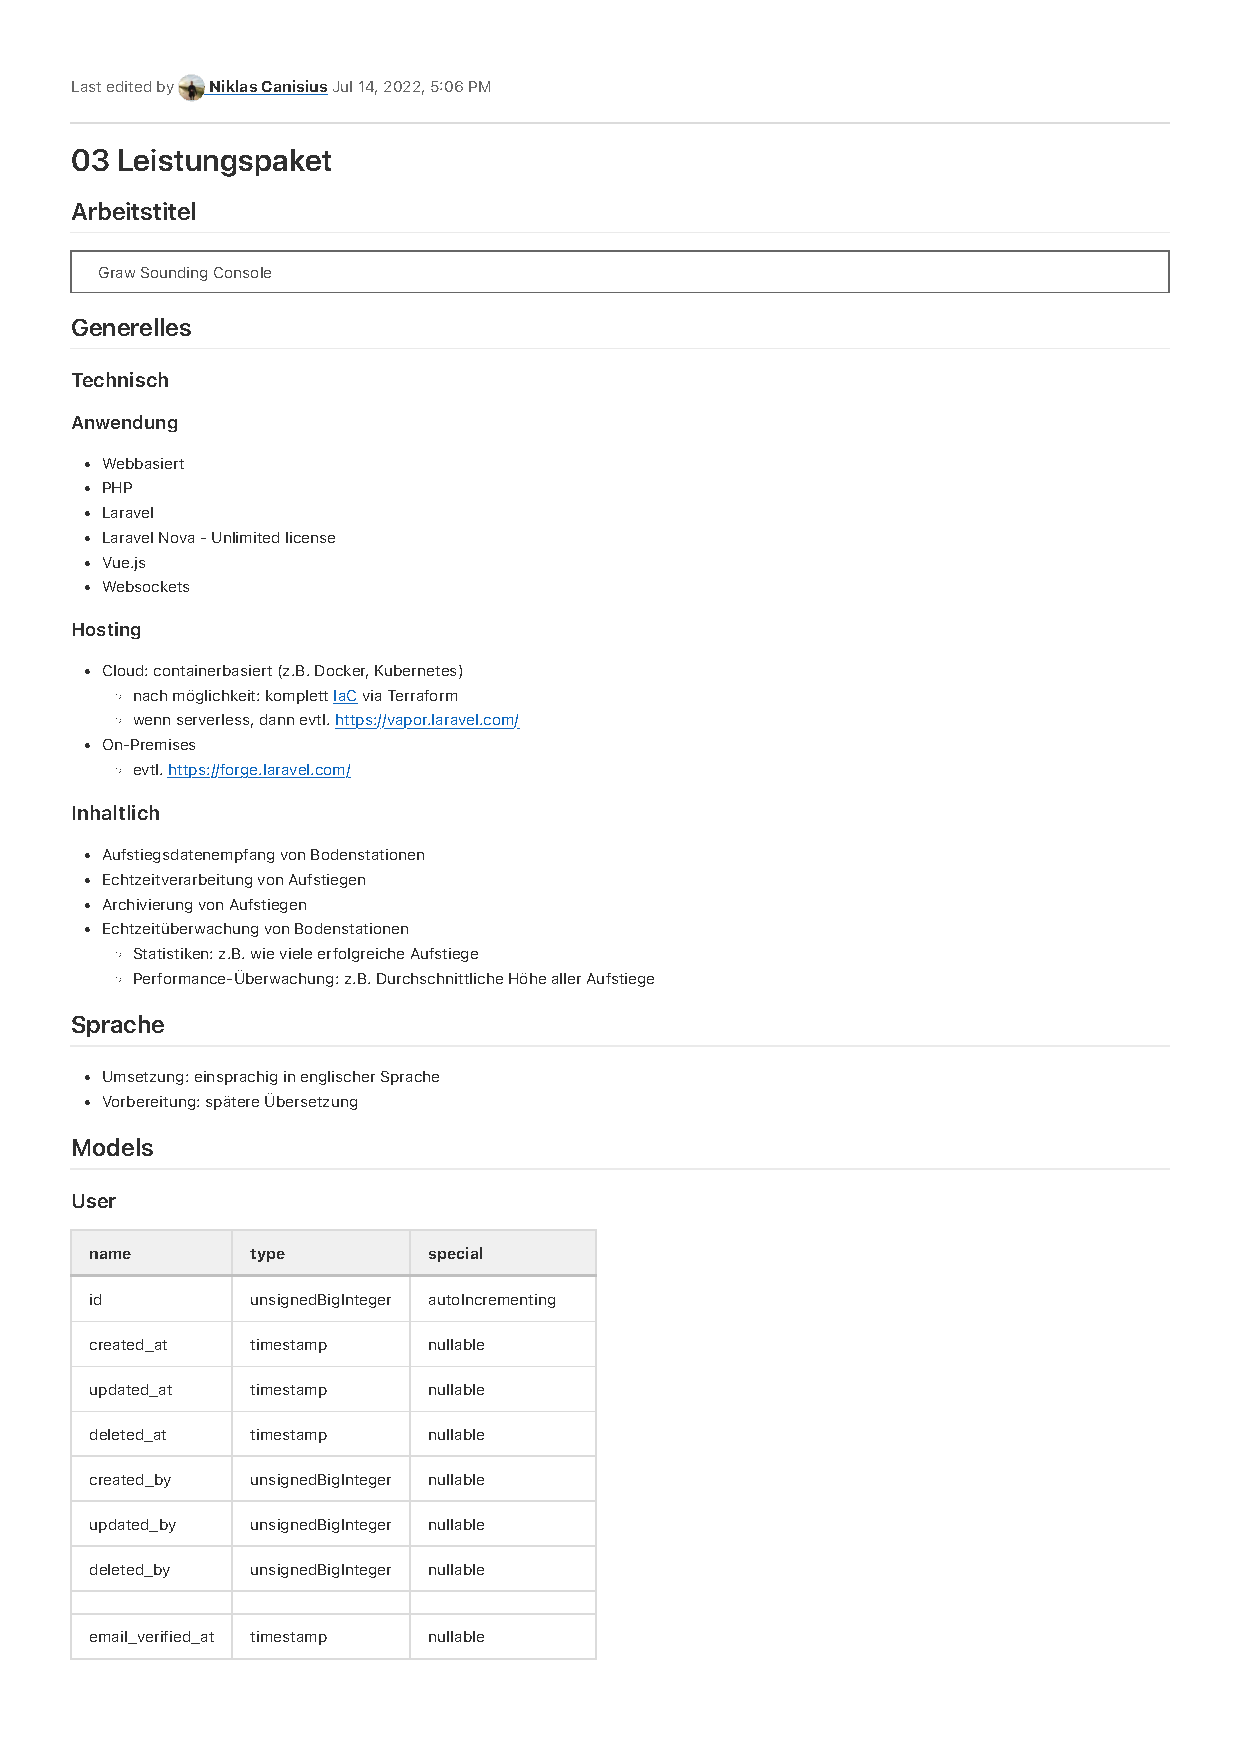
\includepdf[pages=-]{Leistungspaket.pdf}
\end{document}













